%!TEX root = ../thesis.tex
\chapter{盾构隧道服役性能评估方法}

在道路工程领域,同样有对结构服役性能评估的需求,服役性能的影响因素很多,从机理方面研究的出一个综合性的服役性能指标是件困难的事,以往的研究经验表明(Saito和Sinha,\citeyear{saito1991delphi};Kushida等,\citeyear{kushida1997development}),专家打分在实际工程中是可操作性强、效率高的方法。

早在二十世纪六十年代,美国国家公路协会(American Association of State Highway Officials,AASHO)选定了伊利诺伊州、印第安纳州和明尼苏达州的72个沥青混凝土公路段和54个水泥混凝土公路段(AASHO,\citeyear{AASHO1962the}),组织行业专家对所选的路段进行乘车体验和路面观察,之后根据体验和观察结果对公路对进行服役性能打分,评估等级取值为1-5,其中1表示很差,2表示差,3表示一般,4表示好,5表示很好。与此同时,测量和收集与公路服役性能相关的指标,包括路面平整度、车辙深度、裂缝长度和修补面积等。最后通过多元回归方法拟合检测指标值与服役性能评估之间的关系。对于沥青混凝土公路的服役性能$PSI$
\begin{equation}
	\label{equ:psi1}
	PSI=5.03-1.91\log (1+\overline{SV})-1.38{{\overline{RD}}^{2}}-0.01\sqrt{C+P}
\end{equation}
式中:$\overline{SV}$为路面不平整度方差;${{\overline{RD}}^{2}}$为车辙深度平均值;$C$为裂缝长度;$P$为修补面积。对于水泥混凝土公路的服役性能$PSI$
\begin{equation}
	\label{equ:psi2}
	PSI=5.41-1.80\log (1+\overline{SV})-0.09\sqrt{C+P}
\end{equation}

公式\ref{equ:psi1}和公式\ref{equ:psi2}因形式简单,物理意义明确,适合用于日常的公路服役性能评估。在此之后,多位学者在上述数据和公式基础上,或对$PSI$进行修正,或提出新的服役性能指标。如Liu和Herman(\citeyear{liu1996new})研究人为外界激励对公路服役性能的影响,并对$PSI$公式修正以反映路面的真实情况;ASTM(\citeyear{astm20096433})则根据病害劣化程度,采用扣分的方式给出了道路状态指标(PCI)的计算方法;美国其他州的相关部门参照同样的方法,陆续提出合适的服役性能计算公式(Gharaibeh等,\citeyear{gharaibeh2009assessing})。但在盾构隧道领域,并未见有相关的研究。

本章参考美国国家公路协会对路面服役性能评估方法,对盾构隧道进行病害数据采集,专家打分,和打分结果的回归拟合,得出适合盾构隧道的服役性能指标。

%%%%%%%%%%%%%%%%%%%%%%%%%%%%%%%%%%%%%%%%%%%%%%%%%%%%%%%%%%%%%%%%%%%
\section{盾构隧道服役性能定义与假设}

\subsection{盾构隧道服役性能定义}

为了后续更好描述盾构隧道服役性能评估与预测的方法,在本小节先对与盾构隧道服役性能相关的概念,给出其基本定义。

观测变量:由于盾构隧道结构状态变化,而可通过人工检查、全站仪或激光扫描仪等设备测量到可被观测到现象,如隧道纵向沉降、环向收敛和隧道内病害。(Measurable variable: The observable effects that can be measured, either through visual inspection, total stations, or tunnel section scanning devices, of shield tunnel structure condition changes, such as longitudinal settlement, circumferential convergence and distresses.)

解释变量:可用于描述隧道状态变化的不可观测变量。结构的劣化是由一系列解析变量导致的,解释变量包括结构老化、交通情况、环境腐蚀、维护养护措施等。(Explanatory variable: The unobservable fundamental variables that can describe observed phenomena. Structure deterioration is the result of a variety of these variables. For example, age, traffic, environmental erosion, maintenance activities, etc. constitute explanatory variables.)

隧道服役性能:某一区段隧道在当前时间点,保证隧道结构在运营期正常使用和安全运营的能力,不考虑过去或者未来的因素影响。(Tunnel serviceability: The ability of a specific section of the shield tunnel structure to provide normal and safe use in its existing condition on the date of the rating, not on a past date or a future date.)

隧道服役性能评分(TSR):所有专家对隧道服役性能的打分结果平均值。(Tunnel serviceability rating (TSR): The mean of all experts' ratings of tunnel serviceability.)

隧道服役性能指标(TSI):由盾构隧道样本的观测变量组合得到的数学表达式。隧道服役性能指标可用于评估与隧道样本类似的隧道的服役性能。(Tunnel serviceability index (TSI): A mathematical combination of measurable variables obtained from shield tunnel samples. The TSI can be used to evaluate the serviceability of tunnels that are similar to the tunnel samples.)

\subsection{盾构隧道服役性能假设}

隧道服役性能仅考虑当前时间点的隧道状态。这意味着在对隧道评分过程中不考虑隧道过去的状态,因为本文的主要目的是建立隧道服役性能与观测变量之间的数学表达式。如果评分过程考虑过去状态,需要大量的历史数据支持,这在现实当中可操作性低。对于隧道过去和未来的性能状态,后续可通过退化模型进行考虑。

隧道服役性能只与观测变量有关。Ramaswamy(\citeyear{ramaswamy1989estimation})指出观测变量揭示了隧道劣化指标与隧道状态之间的关系,而解析变量则解释了隧道劣化的过程。本章只考虑隧道服役性能,并不考虑隧道性能退化。

%%%%%%%%%%%%%%%%%%%%%%%%%%%%%%%%%%%%%%%%%%%%%%%%%%%%%%%%%%%%%%%%%%%
\section{盾构隧道数据采集}

上海地铁盾构隧道的日常监测、检测项目包括隧道纵向沉降、横向收敛、衬砌管片接缝张开、错台错缝、渗漏水、裂缝、剥落、剥离等,如表\ref{tab:现场调查内容表}所示。目前,沉降与收敛是在隧道建设期间开始,每半年监测一次,渗漏水、裂缝、剥落、接缝张开、错台等病害则在2011年、2012年和2014年进行过三次全线人工检查。

\begin{table}[!htbp]
  \centering
  \caption{盾构隧道现场检查内容表}
    \begin{tabular}{?m{4.19em}"c"m{20.19em}?}
    \thickhline
    \multicolumn{2}{?m{10.13em}<{\centering}"}{调查项目} & \multicolumn{1}{c?}{调查内容} \bigstrut\\
    \thinhline
    \multirow{4}[8]{*}{结构变形} & \multicolumn{1}{m{5.94em}<{\centering}"}{沉降} & \multirow{2}[4]{*}{委托有测量资质单位专项检测} \bigstrut\\
\cline{2-2}    \multicolumn{1}{?c"}{} & \multicolumn{1}{m{5.94em}<{\centering}"}{收敛} & \multicolumn{1}{c?}{} \bigstrut\\
\cline{2-3}    \multicolumn{1}{?c"}{} & \multicolumn{1}{m{5.94em}<{\centering}"}{接缝张开} & 接缝张开位置、接缝张开量 \bigstrut\\
\cline{2-3}    \multicolumn{1}{?c"}{} & \multicolumn{1}{m{5.94em}<{\centering}"}{错台错缝} & 错台位置、错台量 \bigstrut\\
    \thinhline
    \multicolumn{2}{?m{10.13em}<{\centering}"}{渗漏水} & 渗漏点位置、湿润区域形式、湿润区域面积、渗漏状态(喷射、涌流、滴漏、渗漏)、是否混浊、pH值(选测) \bigstrut\\
    \thinhline
    \multicolumn{2}{?m{10.13em}<{\centering}"}{裂缝} & 裂缝的位置、宽度、长度、角度、形状等 \bigstrut\\
    \thinhline
    \multicolumn{2}{?m{10.13em}<{\centering}"}{剥落剥离} & 剥落位置、剥落区域形状、剥落区域面积、剥落深度 \bigstrut\\
    \thickhline
    \end{tabular}%
  \label{tab:现场调查内容表}%
\end{table}%

隧道监测手段有多种,一般可以分为机器检查和人工检查两种。机器检查主要是采用安装在隧道内的无线传感器获取,如渗漏水传感器(程姝菲和黄宏伟,\citeyear{程姝菲2014盾构隧道长期渗漏水检测新方法})、倾角传感器等(何斌等,\citeyear{何斌2013地下隧道变形检测的无线倾角传感器}),或者通过病害采集车(李家平和卢中贺,\citeyear{李家平2016基于盾构隧道激光扫描点云的收敛直径定点计算方法})获取病害图片,通过图像识别方式提取数据。人工检查由检查人员在地铁停运后进入隧道观察记录病害,采用的辅助工具有铅笔、素描底图、塞尺、卷尺、pH试纸、游标卡尺、手电筒、探明灯、数码相机等,如表\ref{tab:盾构隧道现场检查方法}所示。

人工检查病害一般可分为四个步骤:病害观察、类别判定、测量病害和病害记录,由3个人员一组检查,1人负责探照灯照明,1人负责对病害评估、测量和拍照,1人负责记录病害,可以记录在如图\ref{fig:盾构隧道病害检查素描底图}所示的病害素描图上,或者采用手持式iPad记录病害,记录的信息包括上下行、检查日期、病害位置、衬砌环号、病害大致形状等。

\begin{table}[!htbp]
  \centering
  \caption{盾构隧道现场检查方法}
    \begin{tabular}{?m{4.19em}"c"m{7.25em}"m{12.625em}?}
    \thickhline
    \multicolumn{2}{?m{10.005em}<{\centering}"}{调查内容} & \multicolumn{1}{c"}{调查方法}  & \multicolumn{1}{c?}{相关仪器设备} \bigstrut\\
    \thinhline
    \multirow{4}[8]{*}{结构变形} & \multicolumn{1}{m{5.815em}<{\centering}"}{沉降} & \multicolumn{2}{l?}{\multirow{2}[4]{*}{委托有测量资质单位专项检测}} \bigstrut\\
\cline{2-2}    \multicolumn{1}{?l"}{} & \multicolumn{1}{m{5.815em}<{\centering}"}{收敛} & \multicolumn{2}{l?}{} \bigstrut\\
\cline{2-4}    \multicolumn{1}{?l"}{} & \multicolumn{1}{m{5.815em}<{\centering}"}{接缝张开} & 裂缝宽度仪测量 & 裂缝宽度仪、卷尺、素描底图、铅笔 \bigstrut\\
\cline{2-4}    \multicolumn{1}{?l"}{} & \multicolumn{1}{m{5.815em}<{\centering}"}{错台错缝} & 直尺测量  & 直尺、素描底图、铅笔 \bigstrut\\
    \thinhline
    \multicolumn{2}{?m{10.005em}<{\centering}"}{渗漏水} & 素描、室内检测 & pH试纸、室内水质化验、素描底图、铅笔 \bigstrut\\
    \thinhline
    \multicolumn{2}{?m{10.005em}<{\centering}"}{衬砌剥落} & 素描    & 素描底图、铅笔 \bigstrut\\
    \thinhline
    \multicolumn{2}{?m{10.005em}<{\centering}"}{裂缝} & 裂缝宽度仪测量、素描 & 裂缝宽度仪、卷尺、素描底图、铅笔 \bigstrut\\
    \thickhline
    \end{tabular}%
  \label{tab:盾构隧道现场检查方法}%
\end{table}%

\begin{figure}[!h]
    \centering
    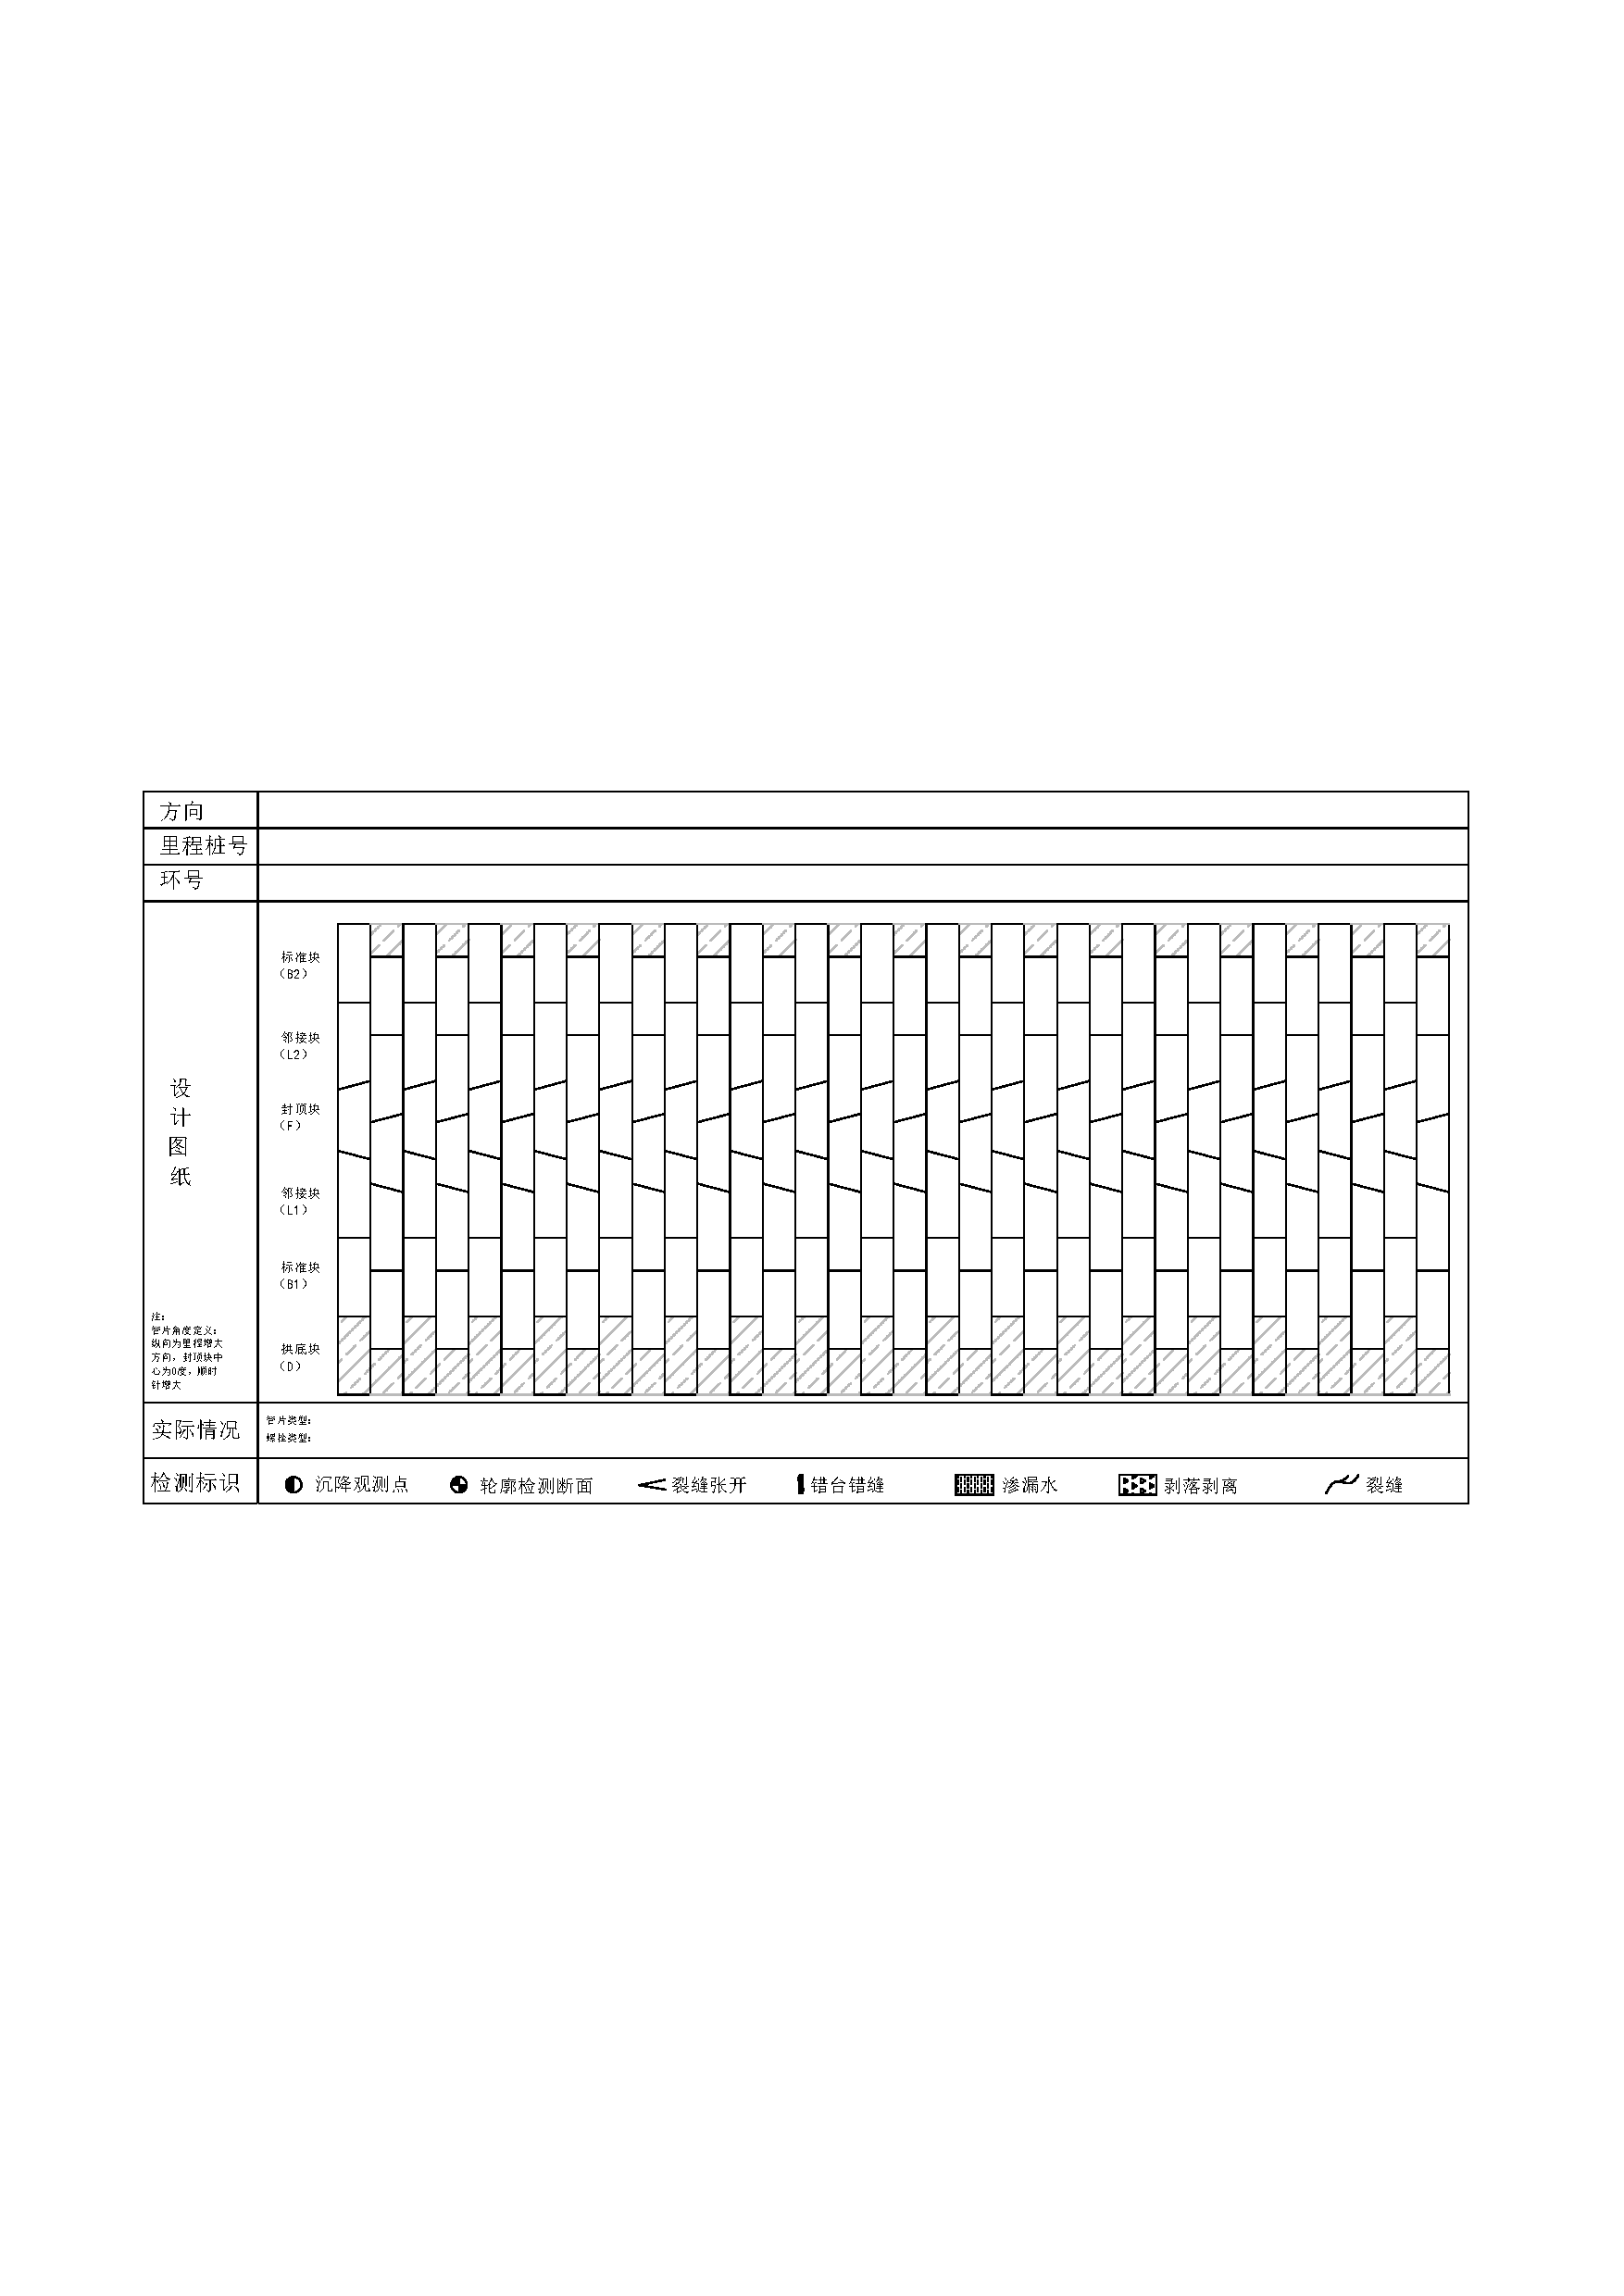
\includegraphics[width=1.0\textwidth]{chap2/distress-check.pdf}
    \caption{盾构隧道病害检查素描底图}
    \label{fig:盾构隧道病害检查素描底图}
\end{figure}

%%%%%%%%%%%%%%%%%%%%%%%%%%%%%%%%%%%%%%%%%%%%%%%%%%%%%%%%%%%%%%%%%%%
\section{盾构隧道服役性能评估指标}

正文




%+++++++++++++++++++++++++++++++++++++++++++++++++++++++++++++++++%
\subsection{沉降}





%+++++++++++++++++++++++++++++++++++++++++++++++++++++++++++++++++%
\subsection{收敛}





%+++++++++++++++++++++++++++++++++++++++++++++++++++++++++++++++++%
\subsection{病害}






%%%%%%%%%%%%%%%%%%%%%%%%%%%%%%%%%%%%%%%%%%%%%%%%%%%%%%%%%%%%%%%%%%%
\section{盾构隧道服役性能评估方法}

正文





%%%%%%%%%%%%%%%%%%%%%%%%%%%%%%%%%%%%%%%%%%%%%%%%%%%%%%%%%%%%%%%%%%%
\section{本章小结}

正文